%!TEX root = ../../main.tex
\chapter{About the Code}\label{app:code}
\partialtoc


%%%%%%%%%%%%%%%%%%%%%%%%%%%%%%%%%%%%%%%%%%%%%%%%%%%%%%%%%%%%%%%%%%%%%%%%%%%%%%%%
%%%%%%%%%%%%%%%%%%%%%%%%%%%%%%%%%%%%%%%%%%%%%%%%%%%%%%%%%%%%%%%%%%%%%%%%%%%%%%%%

\section{Coding the Nonlinear Susceptibility}\label{code}

In this Appendix we reproduce all the quantities  that should be coded.

{\color{red} 
Indeed, in DP \verb=calcolacommutatore.F90=, the expansion coefficients in Eq.
\eqref{forg} are called\\ $E_lf_{lm}^s (\mathbf{K})\to$
\verb=fnlkslm= and $E_l\nabla_\mathbf{K} f_{lm}^s(\mathbf{K})\to$
\verb=fnldkslm=, where \verb=fnlkslm= is an array indexed by
$\mathbf{k}+\mathbf{G}$, and \verb=fnldkslm= is a vector array indexed by
$\mathbf{k}+\mathbf{G}$.}

Eqs.~\eqref{calvimchiewn}, \eqref{calvimchie2wn}, \eqref{calvimchiwn}
 and \eqref{calvimchi2wn}
\begin{equation}\label{calvimchiewn}
\mathrm{Im}[\chi_{e,\mathrm{a}\mathrm{b}\mathrm{c},\omega}^{s,\ell}] =
\frac{\pi |e|^3}{2\hbar^2}\sum_{vc\mathbf{k}}\sum_{l\neq(v,c)}\frac{1}{\omega^\sigma_{cv}}
\left[
\frac{\mathrm{Im}[\mathcal{V}^{\sigma,\text{a},\ell}_{lc}\{r^{\mathrm{b}}_{cv}r^{\mathrm{c}}_{vl}\}]}
{(2\omega^\sigma_{cv}-\omega^\sigma_{cl})} 
-\frac{\mathrm{Im}[\mathcal{V}^{\sigma,\text{a},\ell}_{vl}\{r^{\mathrm{c}}_{lc}r^{\mathrm{b}}_{cv}\}]}
{(2\omega^\sigma_{cv}-\omega^\sigma_{lv})}
\right]\delta(\omega^\sigma_{cv}-\omega),
\end{equation}  
\begin{equation}\label{calvimchiwn}
\mathrm{Im}[\chi_{i,\text{a}\text{b}\text{c},\omega}^{s,\ell}]
= \frac{\pi\vert e\vert^3}{2\hbar^2}\sum_{cv\mathbf{k}}\frac{1}{(\omega^\sigma_{cv})^{2}}
\left[
\mathrm{Re}\left[\left\{r^{\text{b}}_{cv}\left(\mathcal{V}^{\sigma,\text{a},\ell}_{vc}\right)_{;k^{\text{c}}}\right\}\right]
+\frac{\mathrm{Re}\left[\mathcal{V}^{\sigma,\text{a},\ell}_{vc}\left\{r^{\text{b}}_{cv}
\Delta^{\text{c}}_{cv}\right\}\right]}{\omega^\sigma_{cv}} 
\right]\delta(\omega^\sigma_{cv}-\omega),
\end{equation}
\begin{equation}\label{calvimchie2wn}
\mathrm{Im}[\chi_{e,\mathrm{a}\mathrm{b}\mathrm{c},2\omega}^{s,\ell}] =
-\frac{\pi |e|^3}{2\hbar^2}\sum_{vc\mathbf{k}}\frac{4}{\omega^\sigma_{cv}}
\left[
\sum_{v'\ne
  v}\frac{\mathrm{Im}[\mathcal{V}^{\sigma,\text{a},\ell}_{vc}\{r^{\mathrm{b}}_{cv'}r^{\mathrm{c}}_{v'v}\}]}
{2\omega^\sigma_{cv'}-\omega^\sigma_{cv}}
- \sum_{c'\ne
  c}\frac{\mathrm{Im}[\mathcal{V}^{\sigma,\text{a},\ell}_{vc}\{r^{\mathrm{c}}_{cc'}r^{\mathrm{b}}_{c'v}\}]}
{2\omega^\sigma_{c'v}-\omega^\sigma_{cv}}
\right]\delta(\omega^\sigma_{cv}-2\omega),
\end{equation}
and
\begin{equation}\label{calvimchi2wn}
\mathrm{Im}[\chi_{i,\text{a}\text{b}\text{c},2\omega}^{s,\ell}] 
=
 \frac{\pi \vert
   e\vert^{3}}{2\hbar^2}\sum_{vc\mathbf{k}}\frac{4}{(\omega^\sigma_{cv})^{2}}
\left[\mathrm{Re}\left[\mathcal{V}^{\sigma,\text{a},\ell}_{vc}\left\{\left(r^{\text{b}}_{cv}\right)_{;k^{\text{c}}}
\right\}\right] -
\frac{2\mathrm{Re}\left[\mathcal{V}^{\sigma,\text{a},\ell}_{vc}\left\{r^{\text{b}}_{cv}
\Delta^{\text{c}}_{cv}\right\}\right]}{\omega^\sigma_{cv}}\right]\delta(\omega^\sigma_{cv}-2\omega)
,
\end{equation}
\noindent$\bullet$ Coding:
$\mathcal{V}^{\sigma,\mathrm{a},\ell}_{nm}\to$ \verb=calVsig=,
$r^\mathrm{a}_{nm}\to$ \verb=posMatElem=,
$\left(\mathcal{V}^{\sigma,\mathrm{a},\ell}_{nm}\right)_{;k^\mathrm{b}}\to$ \verb=gdcalVsig=,
\\ $(r^\mathrm{a}_{nm})_{;k^\mathrm{b}}\to$ \verb=derMatElem= 
$\Delta^\mathrm{a}_{nm}\to$ \verb=Delta= and $\omega^\sigma_n\to$ \verb=band(n)=

$\bullet$ proof:\\
To evaluate above expressions we need the following ($m_e=1$):
\begin{align}\label{}
\mathbf{v}^\mathrm{LDA}_{nm}(\mathbf{k}) 
=(1/m_e)\mathbf{p}_{nm}(\mathbf{k})+\mathbf{v}^\mathrm{nl}_{nm}(\mathbf{k})
=\mathbf{p}_{nm}(\mathbf{k})+\mathbf{v}^\mathrm{nl}_{nm}(\mathbf{k})
,
\end{align}
that
 includes the local and nonlocal parts of the pseudopotential. They
 correspond to the following files:\\
$\bullet$ $\mathbf{p}_{nm}(\mathbf{k})\to$ \verb=me_pmn_*=\\
$\bullet$ $\mathbf{v}^\mathrm{nl}_{nm}(\mathbf{k})\to$ \verb=me_vnlnm_*=\\
where the \verb=nm= or \verb=mn= order in the files is irrelevant, and
ought to be fixed just for the \emph{biuty} of it.
Option \verb=-n= in \verb=all_responses.sh= does
\begin{enumerate}
\item 
 \verb=> cp me_pmn_* me_pmn_*.o= 
\item adds \verb=me_pmn_*= and \verb=me_vnlnm_*= into
  \verb=me_pmn_*= 
\item calculates the response
\item \verb=> mv me_pmn_*.o me_pmn_*=
\end{enumerate}
so   
$\mathbf{v}^\mathrm{LDA}_{nm}(\mathbf{k})$, stored in \verb=vldaMatElem=
is available for the calculation of the response, and with it we calculate
(Eqs.~\eqref{chon.9} and \eqref{chon.10}),
\begin{align}\label{c-chon.98}
\mathbf{v}^\sigma_{nm}(\mathbf{k})
&=
\left(1+\frac{\Sigma}{\omega_c(\mathbf{k})-\omega_v(\mathbf{k})}\right)\mathbf{v}^\mathrm{LDA}_{nm}(\mathbf{k})
\quad\quad n\notin D_m
\nonumber\\
\mathbf{v}^\sigma_{nn}(\mathbf{k})
&=
\mathbf{v}^\mathrm{LDA}_{nn}(\mathbf{k})
\nonumber\\
\mathbf{r}_{nm}(\mathbf{k})&=\frac{\mathbf{v}^\sigma_{nm}(\mathbf{k})}{i\omega^\sigma_{nm}(\mathbf{k})}
=\frac{\mathbf{v}^\mathrm{LDA}_{nm}(\mathbf{k})}{i\omega^\mathrm{LDA}_{nm}(\mathbf{k})}
\quad\quad n\notin D_m
.
\end{align}   
If option \verb=-n= is not chosen, then the contribution of $\mathbf{v}^\mathrm{nl}_{nm}(\mathbf{k})$
is neglected in the calculation of any response. Obviously, in this
case the code only uses \verb=me_pmn_*= without adding \verb=me_vnlnm_*= 

We need Eq.~\eqref{a.1} and \eqref{a.2}
\begin{align}\label{c-a.1}
\mathcal{V}^{\sigma,\mathrm{a},\ell}_{nm}
&=
\mathcal{V}^{\mathrm{LDA},\mathrm{a},\ell}_{nm}
+
\mathcal{V}^{\mathcal{S},\mathrm{a},\ell}_{nm}
\nonumber\\
\left(
\mathcal{V}^{\sigma,\mathrm{a},\ell}_{nm}
\right)_{;k^\mathrm{b}}
&=
\left(
\mathcal{V}^{\mathrm{LDA},\mathrm{a},\ell}_{nm}
\right)_{;k^\mathrm{b}}
+
\left(
\mathcal{V}^{\mathcal{S},\mathrm{a},\ell}_{nm}
\right)_{;k^\mathrm{b}}
.
\end{align}
 The first LDA term is
\begin{align}\label{c-a.2}
\mathcal{V}^{\mathrm{LDA},\mathrm{a},\ell}_{nm}
&=
\frac{1}{2}\sum_q\left(
v^{\mathrm{LDA},\mathrm{a}}_{nq}\mathcal{C}^\ell_{qm}+\mathcal{C}^\ell_{nq} v^{\mathrm{LDA},\mathrm{a}}_{qm}
\right)
.
\end{align} 
If option \verb=-n= is not chosen in \verb=all_responses.sh=
Eq.~\eqref{c-a.2}
 is
not calculated and\\
$\bullet$ $\mathcal{V}^{\mathrm{LDA},\mathrm{a},\ell}_{nm}\to$ \verb=me_cpmn_*=\\  
If option \verb=-n= is chosen Eq.~\eqref{c-a.2}
 must be calculated as given in
\verb=set_input_ascii.f90=. We mention that
$\mathcal{V}^{\mathrm{LDA},\mathrm{a},\ell}_{nm}$ can be computed directly,\cite{nicolaspc}
avoiding the sum over the full set of bands $q$, however we chose to
compute Eq.~\eqref{c-a.2}, which is done in
\verb=functions.f90= under the name \verb=calVlda=.
Then, we need 
Eq.~\eqref{eni.4}
\begin{align}\label{c-eni.4}
\mathcal{C}^\ell_{nm}(\mathbf{k})&=
\sum_{\mathbf{G},\mathbf{G}'} A^*_{n\mathbf{k}}(\mathbf{G}')  A_{m\mathbf{k}}(\mathbf{G})
\delta_{\mathbf{G}_\parallel \mathbf{G}'_\parallel}
f_\ell(G_\perp-G'_\perp)
\nonumber\\
\mathcal{C}^\ell_{mn}(\mathbf{k})&=
\big(\mathcal{C}^\ell_{nm}(\mathbf{k})\big)^*
,
\end{align} 
which is coded in \verb=sub_pmn_ascii.f90= within the same subroutine of $\boldsymbol{\mathcal{V}}^\ell_{nm}$
calculated with Eq.~\eqref{eni.2}. However, Sean out of the blue, call
it \verb=me_cfmn_*= in \verb=run_tiniba.sh=,
 and Darwin won (what else? ID??), 
thus I call it \verb=cfMatElem= in \verb=SRC_1setinput=. ID would call
it  \verb=ccMatElem=
but long live CD!

 The second LDA term is
\begin{align}\label{c-a.2n}
\left(\mathcal{V}^{\mathrm{LDA},\mathrm{a},\ell}_{nm}\right)_{;k^\mathrm{b}}
&=
\frac{1}{2}\sum_q\left(
(v^{\mathrm{LDA},\mathrm{a}}_{nq})_{;k^\mathrm{b}}\mathcal{C}^\ell_{qm}
+  
v^{\mathrm{LDA},\mathrm{a}}_{nq}(\mathcal{C}^\ell_{qm})_{;k^\mathrm{b}}
+
(\mathcal{C}^\ell_{nq})_{;k^\mathrm{b}} v^{\mathrm{LDA},\mathrm{a}}_{qm}
+
\mathcal{C}^\ell_{nq} (v^{\mathrm{LDA},\mathrm{a}}_{qm})_{;k^\mathrm{b}}
\right)
,
\end{align}  
where\\
$\bullet$ for $n\ne m$\\
Eq.~\eqref{a.3}
\begin{align}\label{c-a.3}
(v^{\mathrm{LDA},\mathrm{a}}_{nm})_{;k^\mathrm{b}}
&=  
im_e\left(\Delta^b_{nm}r^\mathrm{a}_{nm}
+ 
\omega^\mathrm{LDA}_{nm}(r^\mathrm{a}_{nm})_{;k^\mathrm{b}}
\right)
\nonumber\\
(v^{\mathrm{LDA},\mathrm{a}}_{mn})_{;k^\mathrm{b}}
&=
\left((v^{\mathrm{LDA},\mathrm{a}}_{nm})_{;k^\mathrm{b}}\right)^*
\quad\mathrm{for}\quad n\ne m
,
\end{align} 
with
Eq.~\eqref{eli.13}
\begin{align}\label{c-eli.13}
\Delta_{nm}^{\mathrm{a}}
=
v_{nn}^{\mathrm{LDA},\mathrm{a}}-v_{mm}^{\mathrm{LDA},\mathrm{a}}
,
\end{align}
and \eqref{na_rgendevn}
\begin{align}\label{c-na_rgendevn}
(r^{\mathrm{b}}_{nm})_{;k^{\mathrm{a}}}
&=
-i\mathcal{T}^{\mathrm{a}\mathrm{b}}_{nm}
+
\frac{
r^{\mathrm{a}}_{nm}
\Delta^{\mathrm{b}}_{mn}
+r^{\mathrm{b}}_{nm}
\Delta^{\mathrm{a}}_{mn}
}
{\omega^\mathrm{LDA}_{nm}}
+
\frac{i}{\omega^\mathrm{LDA}_{nm}}
\sum_{\ell}
\bigg(
\omega^\mathrm{LDA}_{\ell m}
r^{\mathrm{a}}_{n\ell}
r^{\mathrm{b}}_{\ell m}
-
\omega^\mathrm{LDA}_{n\ell}
r^{\mathrm{b}}_{n\ell}
r^{\mathrm{a}}_{\ell m}
\bigg)
\nonumber\\
&\approx
\frac{
r^{\mathrm{a}}_{nm}
\Delta^{\mathrm{b}}_{mn}
+r^{\mathrm{b}}_{nm}
\Delta^{\mathrm{a}}_{mn}
}
{\omega^\mathrm{LDA}_{nm}}
+
\frac{i}{\omega^\mathrm{LDA}_{nm}}
\sum_{\ell}
\bigg(
\omega^\mathrm{LDA}_{\ell m}
r^{\mathrm{a}}_{n\ell}
r^{\mathrm{b}}_{\ell m}
-
\omega^\mathrm{LDA}_{n\ell}
r^{\mathrm{b}}_{n\ell}
r^{\mathrm{a}}_{\ell m}
\bigg)
\nonumber\\
(r^{\mathrm{b}}_{mn})_{;k^{\mathrm{a}}}
&=
\left((r^{\mathrm{b}}_{nm})_{;k^{\mathrm{a}}}\right)^*
,
\end{align}
where $\mathcal{T}^{\mathrm{a}\mathrm{b}}_{nm}\approx 0$.\\
$\bullet$ for $n=m$\\
Since 
$\mathcal{T}^{\mathrm{a}\mathrm{b}}_{nn}\approx (\hbar/m_e)\delta_{\mathrm{a}\mathrm{b}}$,
Eq.~\eqref{a.3c} gives
\begin{align}\label{c-a.3c}
(v^{\mathrm{LDA},\mathrm{a}}_{nn})_{;k^\mathrm{b}}
&=
-i\mathcal{T}^{\mathrm{a}\mathrm{b}}_{nn}
-
\sum_{\ell\ne n}
\omega^\mathrm{LDA}_{\ell n}
\bigg( 
r^{\mathrm{a}}_{n\ell} 
r^\mathrm{b}_{\ell n}
+ 
r^\mathrm{b}_{n\ell} 
r^{\mathrm{a}}_{\ell n}
\bigg)
\nonumber\\
&\approx
\frac{\hbar}{m_e}\delta_{\mathrm{a}\mathrm{b}}
-
\sum_{\ell\ne n}
\omega^\mathrm{LDA}_{\ell n}
\bigg( 
r^{\mathrm{a}}_{n\ell} 
r^\mathrm{b}_{\ell n}
+ 
r^\mathrm{b}_{n\ell} 
r^{\mathrm{a}}_{\ell n}
\bigg)
.
\end{align} 
For Eq.~\eqref{c-a.2n} we need
\eqref{a.7}
\begin{align}\label{c-a.7}
 (\mathcal{C}^\ell_{nm})_{;k^\mathrm{a}}
&= 
i\sum_{q\ne nm}
\left(
r_{nq}^\mathrm{a}
\mathcal{C}^\ell_{qm}
-
\mathcal{C}^\ell_{nq}
r_{qm}^\mathrm{a}
\right)
+ir_{nm}^\mathrm{a}(\mathcal{C}^\ell_{mm}-\mathcal{C}^\ell_{nn})
\nonumber\\
 (\mathcal{C}^\ell_{mn})_{;\mathbf{k}}
&=
\big( (\mathcal{C}^\ell_{nm})_{;\mathbf{k}}\big)^*
.
\end{align} 

For the scissor related term we have:
Eq.~\eqref{a.3b} , \eqref{choni.1} and \eqref{chon.2}
\begin{align}\label{c-a.3b}
\mathcal{V}^{\mathcal{S},\mathrm{a},\ell}_{nm}
&=
\frac{1}{2}\sum_q\left(    
v^{\mathcal{S},\mathrm{a}}_{nq}\mathcal{C}^\ell_{qm}+\mathcal{C}^\ell_{nq} v^{\mathcal{S},\mathrm{a}}_{qm}
\right)
\nonumber\\
\left(\mathcal{V}^{\mathcal{S},\mathrm{a},\ell}_{nm}\right)_{;k^\mathrm{b}}
&=
\frac{1}{2}\sum_q\left(
(v^{\mathcal{S},\mathrm{a}}_{nq})_{;k^\mathrm{b}}\mathcal{C}^\ell_{qm}
+     
v^{\mathcal{S},\mathrm{a}}_{nq}(\mathcal{C}^\ell_{qm})_{;k^\mathrm{b}}
+
(\mathcal{C}^\ell_{nq})_{;k^\mathrm{b}} v^{\mathcal{S},\mathrm{a}}_{qm}
+
\mathcal{C}^\ell_{nq} (v^{\mathcal{S},\mathrm{a}}_{qm})_{;k^\mathrm{b}}
\right)
,
\end{align}     
with Eqs.~\eqref{chon.2} and \eqref{choni.1}
\begin{align}\label{c-chon.2} 
v^{\mathcal{S},\mathrm{a}}_{nm}=i\Sigma f_{mn}r^\mathrm{a}_{nm}
,
\end{align}
\begin{align}\label{c-choni.1}
(v^{\mathcal{S},\mathrm{a}}_{nm})_{;k^\mathrm{b}}= 
i\Sigma f_{mn}(r^\mathrm{a}_{nm})_{;k^\mathrm{b}}
,
\end{align} 
where $\hbar\Sigma$ is the scissors correction.
Notice that
$v^{\mathcal{S},\mathrm{a}}_{nn}=0$ and 
$(v^{\mathcal{S},\mathrm{a}}_{nn})_{;k^\mathrm{b}}=0$.
Substuiting Eq.~\eqref{c-chon.2} into \eqref{c-a.3b}, we obtain
\begin{align}\label{c-a.3bb}
\mathcal{V}^{\mathcal{S},\mathrm{a},\ell}_{nm}
&=
\frac{i\Sigma}{2}\sum_q\left(  
f_{qn}r^\mathrm{a}_{nq}\mathcal{C}^\ell_{qm}+f_{mq}\mathcal{C}^\ell_{nq} r^\mathrm{a}_{qm}
\right)
,
\end{align}   

$\bullet$ Coding: \verb=functions.f90= array \verb=calVscissors= 
where $f_n$ is coded in \verb=set_input_ascii.f90=\\
Notice that $q=n$ and $q=m$ give zero contribution from the $f_{nm}$
factors, but we set in the code $r^\mathrm{a}_{nn}=0$ so the program would
not complain that such values of the array \verb=posMatElem= do not
exist, since actually, the diagonal elements do not exist.
Explicitly (although, we don't code them), 
\begin{align}\label{vs.vc}
      \mathcal{V}^{S,a,\ell}_{vc}
&= 
      -\frac{i\Sigma}{2}
      \left[\sum_{v^{\prime}}r^{a}_{vv^{\prime}}C^{\ell}_{v^{\prime}c} 
          +
          \sum_{c^{\prime}}C^{\ell}_{vc^{\prime}}r^{a}_{c^{\prime}c}\right],
\nonumber\\
      \mathcal{V}^{S,a,\ell}_{cv}
&= 
      \frac{i\Sigma}{2}
      \left[\sum_{v^{\prime}}r^{a}_{cv^{\prime}}C^{\ell}_{v^{\prime}v} 
          + \sum_{c^{\prime}}C^{\ell}_{cc^{\prime}}r^{a}_{c^{\prime}v}\right],
\nonumber\\
      \mathcal{V}^{S,a,\ell}_{cv}
&= 
      (\mathcal{V}^{S,a,\ell}_{vc})^*
    \end{align}
and    
  \begin{align}\label{vs.cc}
    \mathcal{V}^{S,a,\ell}_{cc} 
    &= -\Sigma\sum_{v}
    \text{Im}\left[r^{a}_{cv}C^{\ell}_{vc}\right],
  \end{align}
 \begin{align}\label{vs.vv}
    \mathcal{V}^{S,a,\ell}_{vv} 
    &= \Sigma\sum_{c}
    \text{Im}\left[r^{a}_{vc}C^{\ell}_{cv}\right],
  \end{align}
where the last two are real functions as they must, since they are
velocities. 

Substuiting Eqs.~\eqref{c-chon.2} and \eqref{c-choni.1} into \eqref{c-a.3b}, we obtain
\begin{align}\label{c-a.3bnn}
\left(\mathcal{V}^{\mathcal{S},\mathrm{a},\ell}_{nm}\right)_{;k^\mathrm{b}}
&=
\frac{i\Sigma}{2}\sum_q\left(
f_{qn}\Big[
(r^\mathrm{a}_{nq})_{;k^\mathrm{b}}\mathcal{C}^\ell_{qm}
+    
r^\mathrm{a}_{nq}(\mathcal{C}^\ell_{qm})_{;k^\mathrm{b}}
\Big]
+
f_{mq}\Big[
(\mathcal{C}^\ell_{nq})_{;k^\mathrm{b}} r^\mathrm{a}_{qm}
+
\mathcal{C}^\ell_{nq} (r^\mathrm{a}_{qm})_{;k^\mathrm{b}}
\Big]
\right)
\nonumber\\
\left(\mathcal{V}^{\mathcal{S},\mathrm{a},\ell}_{mn}\right)_{;k^\mathrm{b}}
&=
\left(\left(\mathcal{V}^{\mathcal{S},\mathrm{a},\ell}_{nm}\right)_{;k^\mathrm{b}}\right)^*
,
\end{align}    
$\bullet$ Coding:\\
$(r^\mathrm{a}_{nm})_{;k^\mathrm{b}}\to$ \verb=derMatElem=
$\mathcal{C}^\ell_{nm}\to$ \verb=cfMatElem=
$r^\mathrm{a}_{nm}\to$ \verb=posMatElem=
$(\mathcal{C}^\ell_{nm})_{;k^\mathrm{b}}\to$ \verb=gdf=, and\\
$\left(\mathcal{V}^{\mathcal{S},\mathrm{a},\ell}_{nm}\right)_{;k^\mathrm{b}}\to$ 
\verb=gdcalVS=\\
Also
\begin{align}\label{dgvs.cv}
\left(\mathcal{V}^{\mathcal{S},\mathrm{a}\,\ell}_{cv}\right)_{;k^\mathrm{b}}
&=
\frac{i\Sigma}{2}
\left(
\sum_{v'}\left(
 (r^\mathrm{a}_{cv'})_{;k^\mathrm{b}}\mathcal{C}^\ell_{v'v}
+  
r^\mathrm{a}_{cv'}(\mathcal{C}^\ell_{v'v})_{;k^\mathrm{b}}
\right)
+
\sum_{c'}\left(
(\mathcal{C}^\ell_{cc'})_{;k^\mathrm{b}} r^\mathrm{a}_{c'v}
+
\mathcal{C}^\ell_{cc'} (r^\mathrm{a}_{c'v})_{;k^\mathrm{b}}
\right)
\right)
\nonumber\\
\left(\mathcal{V}^{\mathcal{S},\mathrm{a},\ell}_{vc}\right)_{;k^\mathrm{b}}
&=
\left(\left(\mathcal{V}^{\mathcal{S},\mathrm{a},\ell}_{cv}\right)_{;k^\mathrm{b}}\right)^*
,
\end{align}  
\begin{align}\label{dgvs.cc}
\left(\mathcal{V}^{\mathcal{S},\mathrm{a},\ell}_{cc}\right)_{;k^\mathrm{b}}
&=
-\Sigma
\sum_{v}
 \mathrm{Im}\left[(r^\mathrm{a}_{cv})_{;k^\mathrm{b}}\mathcal{C}^\ell_{vc}
+
r^\mathrm{a}_{cv}
(\mathcal{C}^\ell_{vc}) _{;k^\mathrm{b}}\right]
,
\end{align}  
and
\begin{align}\label{dgvs.vv}
\left(\mathcal{V}^{\mathcal{S},\mathrm{a},\ell}_{vv}\right)_{;k^\mathrm{b}}
&=
\Sigma
\sum_{c}
 \mathrm{Im}\left[(r^\mathrm{a}_{vc})_{;k^\mathrm{b}}\mathcal{C}^\ell_{cv}
+
r^\mathrm{a}_{vc}(\mathcal{C}^\ell_{cv}) _{;k^\mathrm{b}}\right]
.
\end{align}  

%%%%%%%%%%%%%%%%%%%%%%%%%%%%%%%%%%%%%%%%%%%%%%%%%%%%%%%%%%%%%%%%%%%%%%%%%%%%%%%%


\subsection{Coding for \texorpdfstring{$\mathcal{V}^{\sigma,\mathrm{a},\ell}_{nm}(\mathbf{k})$}{Vnm}} 

Recall that 
$\mathcal{V}^{\mathrm{LDA},\mathrm{a},\ell}_{mn}=(\mathcal{V}^{\mathrm{LDA},\mathrm{a},\ell}_{nm})^*$
and 
$\mathcal{V}^{\mathcal{S},\mathrm{a},\ell}_{mn}=(\mathcal{V}^{\mathcal{S},\mathrm{a},\ell}_{nm})^*$ 
\begin{itemize}
%%%
\item If \verb=-n= option is chosen in \verb=all_responses.sh=
\begin{itemize}
\item $\mathcal{V}^{\mathrm{LDA},\mathrm{a},\ell}_{nm}$, comes from
  Eq.~\eqref{c-a.2}, coded in \verb=functions.f90= as \verb=calVlda=
\end{itemize}
%%%
\item If \verb=-n= option is NOT chosen in \verb=all_responses.sh=
\begin{itemize}
\item $\mathcal{V}^{\mathrm{LDA},\mathrm{a},\ell}_{nm}$ 
is used from \verb=me_cpmn_*=
  which is Eq.~\eqref{eni.2} and is coded in \verb=sub_pmn_ascii.f90=
\end{itemize}
%%%
\end{itemize}
For either case
\begin{itemize}
\item $\mathcal{V}^{\mathcal{S},\mathrm{a},\ell}_{nm}$ 
is obtained from
  Eqs.~\eqref{vs.vc}, \eqref{vs.cc} or \eqref{vs.vv}, depending on
  $nm$. This is coded in \verb=functions.f90= and used in 
\verb=set_input_ascii.f90=  
\end{itemize}
Thus,\\
$\bullet$ 
$\mathcal{V}^{\sigma,\mathrm{a},\ell}_{nm}(\mathbf{k})=\mathcal{V}^{\mathrm{LDA},\mathrm{a},\ell}_{nm}(\mathbf{k})+\mathcal{V}^{\mathcal{S},\mathrm{a},\ell}_{nm}(\mathbf{k})$\\ 
is stored in \verb=calMomMatElem=  
array, constructed in 
\verb=set_input_ascii.f90=, and used in \verb=SRC_2latm= for
integrating the response function. A brave young soul, should change   
\verb=calMomMatElem= to \verb=calVelMatElem= in order to have a more
appropriate name. But as good old DNA, we construct upon available
ATGC; using the old structure, adding functionality and  keeping all
the usles non-codifying crap, thus making Darwin
 proud of us! 


%%%%%%%%%%%%%%%%%%%%%%%%%%%%%%%%%%%%%%%%%%%%%%%%%%%%%%%%%%%%%%%%%%%%%%%%%%%%%%%%

\subsection{Coding \texorpdfstring{$\Delta^{\sigma,\mathrm{a},\ell}_{nm}(\mathbf{k})$}{Deltanm}}

$\Delta^{\sigma,\mathrm{a},\ell}_{nm}(\mathbf{k})$  is given by
\begin{align}\label{caldelta}
\Delta^{\sigma,\mathrm{a},\ell}_{nm}(\mathbf{k})&=\mathcal{V}^{\sigma,\mathrm{a},\ell}_{nn}(\mathbf{k})-\mathcal{V}^{\sigma,\mathrm{a},\ell}_{mm}(\mathbf{k})
\end{align}
\begin{align}\label{delta}
\Delta^{\sigma,\mathrm{a}}_{nm}(\mathbf{k}) &=v^{\sigma,\mathrm{a},\ell}_{nn}(\mathbf{k})-v^{\sigma,\mathrm{a},\ell}_{mm}(\mathbf{k})
\nonumber\\
&=v^{\mathrm{LDA},\mathrm{a},\ell}_{nn}(\mathbf{k})-v^{\mathrm{LDA},\mathrm{a},\ell}_{mm}(\mathbf{k})
,
\end{align}
since $\mathbf{v}^\mathcal{S}_{nn}=0$.\\
$\bullet$ Coding: $\Delta^{\sigma,\mathrm{a},\ell}_{nm}(\mathbf{k})\to$ \verb=calDelta= 
and
$\Delta^{\sigma,\mathrm{a}}_{nm}(\mathbf{k})\to$ \verb=Delta= both in \verb=set_input_ascii.f90= 


%%%%%%%%%%%%%%%%%%%%%%%%%%%%%%%%%%%%%%%%%%%%%%%%%%%%%%%%%%%%%%%%%%%%%%%%%%%%%%%%

\subsection{Coding for \texorpdfstring{$(\mathcal{V}^{\mathrm{LDA},\mathrm{a},\ell}_{nm}(\mathbf{k}))_{;k^\mathrm{b}}$}{(Vnm);k}}
\begin{itemize}
\item $\Delta^\mathrm{a}_{nm}$ available in array \verb=Delta=, 
calculated in \verb=set_input_ascii.f90=,
 and contains the
  contribution from $\mathbf{v}^\mathrm{nl}_{nm}(\mathbf{k})$ if the \verb=-n= option is
  chosen in \verb=all_responses.sh= 
\item $(r^\mathrm{a}_{nm}(\mathbf{k}))_{;k^\mathrm{b}}$
 available in array
  \verb=derMatElem=,
calculated in \verb=set_input_ascii.f90= and \verb=functions.f90=,
 and contains the
  contribution from $\mathbf{v}^\mathrm{nl}_{nm}(\mathbf{k})$ if the \verb=-n= option is
  chosen in \verb=all_responses.sh= 
\item With above two we compute $(v^{\mathrm{LDA},\mathrm{a}}_{nm}(\mathbf{k}))_{;k^\mathrm{b}}$ 
in \verb=set_input_ascii.f90=  and store it in \verb=gdVlda= for
diagonal and off diagonal terms.
\item $\big(\mathcal{C}^\ell_{nm}(\mathbf{k})\big)_{;k^\mathrm{a}}$ is coded in 
in \verb=set_input_ascii.f90=  and store it in \verb=gdf= for
diagonal and off diagonal terms. Darwin at work!
\item $(v^{\mathrm{LDA},\mathrm{a}}_{nq})_{;k^\mathrm{b}}\to$ \verb=gdVlda=,
  $\mathcal{C}^\ell_{qm}\to$ \verb=cfMatElem=,
$v^{\mathrm{LDA},\mathrm{a}}_{nq}\to$ \verb=vldaMatElem=, 
$(\mathcal{C}^\ell_{qm})_{;k^\mathrm{b}}\to$
\verb=gdf=\\
 $v^{\mathrm{LDA},\mathrm{a}}_{nq}\to$ \verb=vldaMatElem=,

 \begin{align}\label{c-a.2nn}
\left(\mathcal{V}^{\mathrm{LDA},\mathrm{a},\ell}_{nm}\right)_{;k^\mathrm{b}}
&=
\frac{1}{2}\sum_q\left(
(v^{\mathrm{LDA},\mathrm{a}}_{nq})_{;k^\mathrm{b}}\mathcal{C}^\ell_{qm}
+ 
v^{\mathrm{LDA},\mathrm{a}}_{nq}(\mathcal{C}^\ell_{qm})_{;k^\mathrm{b}}
+
(\mathcal{C}^\ell_{nq})_{;k^\mathrm{b}} v^{\mathrm{LDA},\mathrm{a}}_{qm}
+
\mathcal{C}^\ell_{nq} (v^{\mathrm{LDA},\mathrm{a}}_{qm})_{;k^\mathrm{b}}
\right)
\nonumber\\
\left(\mathcal{V}^{\mathrm{LDA},\mathrm{a},\ell}_{mn}\right)_{;k^\mathrm{b}}&=\left(\left(\mathcal{V}^{\mathrm{LDA},\mathrm{a},\ell}_{nm}\right)_{;k^\mathrm{b}}\right)^*
,
\end{align} 
$\left(\mathcal{V}^{\mathrm{LDA},\mathrm{a},\ell}_{nm}\right)_{;k^\mathrm{b}}\to$
\verb=gdcalVlda= and coded in \verb=set_input_ascii.f90=
\end{itemize}


%%%%%%%%%%%%%%%%%%%%%%%%%%%%%%%%%%%%%%%%%%%%%%%%%%%%%%%%%%%%%%%%%%%%%%%%%%%%%%%%

\subsection{Summary}
\begin{itemize}
\item
$\mathcal{V}^{\sigma,\mathrm{a},\ell}_{nm}(\mathbf{k})=\mathcal{V}^{\mathrm{LDA},\mathrm{a},\ell}_{nm}(\mathbf{k})+\mathcal{V}^{\mathcal{S},\mathrm{a},\ell}_{nm}(\mathbf{k})\to$
\verb=calMomMatElem= 

\item $\left(\mathcal{V}^{\mathrm{LDA},\mathrm{a},\ell}_{nm}\right)_{;k^\mathrm{b}}\to$
\verb=gdcalVlda= 

\item $\left(\mathcal{V}^{\mathcal{S},\mathrm{a},\ell}_{nm}\right)_{;k^\mathrm{b}}\to$ 
\verb=gdcalVS=

\item $\left(\mathcal{V}^{\sigma,\mathrm{a},\ell}_{nm}\right)_{;k^\mathrm{b}}=
\left(\mathcal{V}^{\mathrm{LDA},\mathrm{a},\ell}_{nm}\right)_{;k^\mathrm{b}}+\left(\mathcal{V}^{\mathcal{S},\mathrm{a},\ell}_{nm}\right)_{;k^\mathrm{b}}\to$ 
\verb=gdcalVsig=
\end{itemize}


%%%%%%%%%%%%%%%%%%%%%%%%%%%%%%%%%%%%%%%%%%%%%%%%%%%%%%%%%%%%%%%%%%%%%%%%%%%%%%%%

\subsection{Bulk expressions}

For a bulk $\mathcal{C}^\ell_{nm}(\mathbf{k})=\delta_{nm}$, then
$(\mathcal{C}^\ell_{nm}(\mathbf{k}))_{;\mathbf{k}}=0$, and Eq.~\eqref{c-a.1} reduces to
\begin{align}\label{choni.9}
v^{\sigma,\mathrm{a}}_{nm}
&=
v^{\mathrm{LDA},\mathrm{a}}_{nm}
+
v^{\mathcal{S},\mathrm{a}}_{nm}
\nonumber\\
\mathbf{v}^\sigma_{nm}(\mathbf{k})
&=
\left(1+\frac{\Sigma}{\omega_c(\mathbf{k})-\omega_v(\mathbf{k})}\right)\mathbf{v}^\mathrm{LDA}_{nm}(\mathbf{k})
\quad\quad n\notin D_m
\nonumber\\
\mathbf{v}^\sigma_{nn}(\mathbf{k})
&=
\mathbf{v}^\mathrm{LDA}_{nn}(\mathbf{k})
,
\end{align}
where in \verb=$TINIBA/latm= the values are coded in the array
called
\verb=momMatElem=.  
If option \verb=-n= is given while running
\verb=all_resposnses.sh=, then $\mathbf{v}^\mathrm{nl}_{nm}(\mathbf{k})$ are included in 
\verb=momMatElem=. 
Also,
\begin{align}\label{c-a.1nn}
\left(v^{\sigma,\mathrm{a}}_{nm}\right)_{;k^\mathrm{b}}
&=
\left(
v^{\mathrm{LDA},\mathrm{a}}_{nm}
\right)_{;k^\mathrm{b}}
+
\left(
v^{\mathcal{S},\mathrm{a}}_{nm}
\right)_{;k^\mathrm{b}}
\nonumber\\
&=
\left(
v^{\mathrm{LDA},\mathrm{a}}_{nm}
\right)_{;k^\mathrm{b}}
+
i\Sigma f_{mn}(r^\mathrm{a}_{nm})_{;k^\mathrm{b}}
\nonumber\\
\left(v^{\sigma,\mathrm{a}}_{mn}\right)_{;k^\mathrm{b}}
&=
\left(\left(v^{\sigma,\mathrm{a}}_{nm}\right)_{;k^\mathrm{b}}\right)^*
,
\end{align}
where with the r.h.s. expressions are given above. 

$\bullet$ Coding:
$\mathbf{v}^\sigma_{nm}(\mathbf{k})\to$ \verb=momMatElem=,
$\left(v^{\mathrm{LDA},\mathrm{a}}_{nm}\right)_{;k^\mathrm{b}}\to$ \verb=gdVlda=,
$\left(r^{\mathrm{LDA},\mathrm{a}}_{nm}\right)_{;k^\mathrm{b}}\to$ \verb=derMatElem=, and
$\left(v^{\sigma,\mathrm{a}}_{nm}\right)_{;k^\mathrm{b}}\to$ \verb=gdVsig=


%%%%%%%%%%%%%%%%%%%%%%%%%%%%%%%%%%%%%%%%%%%%%%%%%%%%%%%%%%%%%%%%%%%%%%%%%%%%%%%%

\subsection{Calculating a layer or bulk response}

\begin{itemize}
\item Layer: The layer calculation is done by using
Eqs.~\eqref{c-calvimchiewn}, \eqref{c-calvimchie2wn}, \eqref{c-calvimchiwn}
 and \eqref{c-calvimchi2wn}. 
\item Bulk:
A bulk calculation can be performed by using the same
Eqs.~\eqref{c-calvimchiewn}, \eqref{c-calvimchie2wn}, \eqref{c-calvimchiwn}
 and \eqref{c-calvimchi2wn}, and by simply replacing
\begin{enumerate}
\item $\boldsymbol{\mathcal{V}}^\sigma_{nm}$ (\verb=calMomMatElem=) $\to \mathbf{v}^\sigma_{nm}$ (\verb=momMatElem=) 
\item $(\boldsymbol{\mathcal{V}}^\sigma_{nm})_{;\mathbf{k}}$ (\verb=gdcalVsig=) $\to
  (\mathbf{v}^\sigma_{nm})_{;\mathbf{k}}$ (\verb=gdVsig=) 
\end{enumerate}
\item Therefore: For the code to run either possibility we use the
  same arrays as for the layered response, where, if bulk is chosen, it
  simply copies the bulk matrix elements into the layer arrays, i.e.
\begin{itemize}
\item Layer: 
$\boldsymbol{\mathcal{V}}^\sigma_{nm}$ (\verb=calMomMatElem=) and
$(\boldsymbol{\mathcal{V}}^\sigma_{nm})_{;\mathbf{k}}$ (\verb=gdcalVsig=) 
\item Bulk:
$\mathbf{v}^\sigma_{nm}$ (\verb=momMatElem=$\to$\verb=calVsig=) and
$(\mathbf{v}^\sigma_{nm})_{;\mathbf{k}}$ (\verb=gdVsig=$\to$\verb=gdcalVsig=) \\
This change is done in \verb=set_input_ascii.f90= (look for
\verb=layer-to-bulk= tag)
\item ID: Notice that we have assigned\\
  \verb=calMomMatElem=$\to$ \verb=calVsig= (keeping
  \verb=calMomMatElem=), so it is easier to  code the responses.
Therefore, we have\\
$\boldsymbol{\mathcal{V}}^\sigma_{nm}\to$ \verb=calVsig= and
$(\boldsymbol{\mathcal{V}}^\sigma_{nm})_{;\mathbf{k}}\to$ \verb=gdcalVsig=\\
either for bulk or layered response. \\
If \verb=calMomMatElem= is not used, we should get rid of it (ID at work).
\end{itemize}
\end{itemize}


%%%%%%%%%%%%%%%%%%%%%%%%%%%%%%%%%%%%%%%%%%%%%%%%%%%%%%%%%%%%%%%%%%%%%%%%%%%%%%%%

\subsection{\texorpdfstring{$\mathcal{V}$ vs $\mathcal{R}$}{V vs R}}

Using 
$\mathrm{Re}[iz]=-\mathrm{Im}[z]$,
$\mathrm{Im}[iz]=\mathrm{Re}[z]$,
and
\begin{equation}\label{rnmenm91}
\mathcal{R}^\mathrm{a}_{nm}=\frac{\mathcal{P}^\mathrm{a}_{nm}}{im_e\omega_{nm}}=\frac{\mathcal{V}^\mathrm{a}_{nm}}{i\omega_{nm}}
\quad\quad n\ne m
,
\end{equation}
we can show the equivalence between the two formulations, i.e.
\begin{align}\label{imchiew}
\mathrm{Im}[\chi_{e,\mathrm{a}\mathrm{b}\mathrm{c},\omega}^{s,\ell}]
&=
\frac{\pi |e|^3}{2\hbar^2} 
\sum_{vc\mathbf{k}}
\sum_{l\neq(v,c)}
\left[
\frac{\omega^S_{lc}\mathrm{Re}[\mathcal{R}^{\mathrm{a},\ell}_{lc}\{r^{\mathrm{b}}_{cv}r^{\mathrm{c}}_{vl}\}]}
{\omega^S_{cv}(2\omega^S_{cv}-\omega^S_{cl})}
-
\frac{\omega^S_{vl}\mathrm{Re}[\mathcal{R}^{\mathrm{a},\ell}_{vl}\{r^{\mathrm{c}}_{lc}r^{\mathrm{b}}_{cv}\}]}
{\omega^S_{cv}(2\omega^S_{cv}-\omega^S_{lv})}
\right]
\delta(\omega^S_{cv}-\omega)
,
\end{align}  
\begin{equation}\label{c-calvimchiewn}
\mathrm{Im}[\chi_{e,\mathrm{a}\mathrm{b}\mathrm{c},\omega}^{s,\ell}] =
\frac{\pi |e|^3}{2\hbar^2}\sum_{vc\mathbf{k}}\sum_{l\neq(v,c)}\frac{1}{\omega^{S}_{cv}}
\left[
\frac{\mathrm{Im}[\mathcal{V}^{\sigma,\text{a},\ell}_{lc}\{r^{\mathrm{b}}_{cv}r^{\mathrm{c}}_{vl}\}]}
{(2\omega^\sigma_{cv}-\omega^\sigma_{cl})} 
-\frac{\mathrm{Im}[\mathcal{V}^{\sigma,\text{a},\ell}_{vl}\{r^{\mathrm{c}}_{lc}r^{\mathrm{b}}_{cv}\}]}
{(2\omega^\sigma_{cv}-\omega^\sigma_{lv})}
\right]\delta(\omega^\sigma_{cv}-\omega),
\end{equation}  
\begin{align}\label{imchiwf}
\mathrm{Im}[\chi_{i,\mathrm{a}\mathrm{b}\mathrm{c},\omega}^{s,\ell}]
&=
\frac{\pi|e|^3}{2\hbar^2}
\sum_{cv\mathbf{k}}
\frac{1}{\omega^S_{cv}}
\left[
\mathrm{Im}[\{r^{\mathrm{b}}_{cv}\left(\mathcal{R}^{\mathrm{a},\ell}_{vc}\right)_{;k^{\mathrm{c}}}\}]
+
\frac{2\mathrm{Im}[\mathcal{R}^{\mathrm{a},\ell}_{vc}\{r^{\mathrm{b}}_{cv}\Delta^{\mathrm{c}}_{cv}\}]}{\omega^S_{cv}}
\right]
\delta(\omega^S_{cv}-\omega)
,
\end{align}
\begin{equation}\label{c-calvimchiwn}
\mathrm{Im}[\chi_{i,\text{a}\text{b}\text{c},\omega}^{s,\ell}]
= \frac{\pi\vert e\vert^3}{2\hbar^2}\sum_{cv\mathbf{k}}\frac{1}{(\omega^{S}_{cv})^{2}}
\left[
\mathrm{Re}\left[\left\{r^{\text{b}}_{cv}\left(\mathcal{V}^{\sigma,\text{a},\ell}_{vc}\right)_{;k^{\text{c}}}\right\}\right]
+\frac{\mathrm{Re}\left[\mathcal{V}^{\sigma,\text{a},\ell}_{vc}\left\{r^{\text{b}}_{cv}
\Delta^{\text{c}}_{cv}\right\}\right]}{\omega^{S}_{cv}} 
\right]\delta(\omega^\sigma_{cv}-\omega),
\end{equation}
\begin{align}\label{imchie2w}
\mathrm{Im}[\chi_{e,\mathrm{a}\mathrm{b}\mathrm{c},2\omega}^{s,\ell}]
&=
\frac{\pi |e|^3}{2\hbar^2} 
\sum_{vc\mathbf{k}} 
4
\left[
\sum_{v'\ne v}
\frac{\mathrm{Re}[\mathcal{R}^{\mathrm{a},\ell}_{vc}\{r^{\mathrm{b}}_{cv'}r^{\mathrm{c}}_{v'v}\}]}{2\omega^S_{cv'}-\omega^S_{cv}}
-
\sum_{c'\ne c}
\frac{\mathrm{Re}[\mathcal{R}^{\mathrm{a},\ell}_{vc}\{r^{\mathrm{c}}_{cc'}r^{\mathrm{b}}_{c'v}\}]}
{2\omega^S_{c'v}-\omega^S_{cv}}
\right]
\delta(\omega^S_{cv}-2\omega)
,
\end{align}  
\begin{equation}\label{c-calvimchie2wn}
\mathrm{Im}[\chi_{e,\mathrm{a}\mathrm{b}\mathrm{c},2\omega}^{s,\ell}] =
-\frac{\pi |e|^3}{2\hbar^2}\sum_{vc\mathbf{k}}\frac{4}{\omega^{S}_{cv}}
\left[
\sum_{v'\ne
  v}\frac{\mathrm{Im}[\mathcal{V}^{\sigma,\text{a},\ell}_{vc}\{r^{\mathrm{b}}_{cv'}r^{\mathrm{c}}_{v'v}\}]}
{2\omega^\sigma_{cv'}-\omega^\sigma_{cv}}
- \sum_{c'\ne
  c}\frac{\mathrm{Im}[\mathcal{V}^{\sigma,\text{a},\ell}_{vc}\{r^{\mathrm{c}}_{cc'}r^{\mathrm{b}}_{c'v}\}]}
{2\omega^\sigma_{c'v}-\omega^\sigma_{cv}}
\right]\delta(\omega^\sigma_{cv}-2\omega),
\end{equation}
 and
\begin{align}\label{imchi2wf}
\mathrm{Im}[\chi_{i,\mathrm{a}\mathrm{b}\mathrm{c},2\omega}^{s,\ell}]
&=
\frac{\pi|e|^3}{2\hbar^2}\sum_{vc\mathbf{k}}
\frac{4}{\omega^S_{cv}}
\left[
\mathrm{Im}[\mathcal{R}^{\mathrm{a},\ell}_{vc}\{\left(r^{\mathrm{b}}_{cv}\right)_{;k^{\mathrm{c}}}\}]
-
\frac{2\mathrm{Im}[\mathcal{R}^{\mathrm{a},\ell}_{vc}\{r^{\mathrm{b}}_{cv}\Delta^{\mathrm{c}}_{cv}\}]}{\omega^S_{cv}}
\right]\delta(\omega^S_{cv}-2\omega)
,
\end{align}
\begin{equation}\label{c-calvimchi2wn}
\mathrm{Im}[\chi_{i,\text{a}\text{b}\text{c},2\omega}^{s,\ell}] 
=
 \frac{\pi \vert
   e\vert^{3}}{2\hbar^2}\sum_{vc\mathbf{k}}\frac{4}{(\omega^{S}_{cv})^{2}}
\left[\mathrm{Re}\left[\mathcal{V}^{\sigma,\text{a},\ell}_{vc}\left\{\left(r^{\text{b}}_{cv}\right)_{;k^{\text{c}}}
\right\}\right] -
\frac{2\mathrm{Re}\left[\mathcal{V}^{\sigma,\text{a},\ell}_{vc}\left\{r^{\text{b}}_{cv}
\Delta^{\text{c}}_{cv}\right\}\right]}{\omega^{S}_{cv}}\right]\delta(\omega^\sigma_{cv}-2\omega)
,
\end{equation}
\noindent If we take $\mathcal{R}^{\mathrm{a},\ell}_{nm}\to r^\mathrm{a}_{nm}$, 
we
would recover the expressions for a bulk response.
We prefer to use the expressions in terms of $\mathcal{V}^\ell$, since they are
more physically appealing, as the velocity is what gives the current
of a given layer, from which the polarization is computed and the
$\chi^\ell$ extracted.   

{\color{red} Remark:} We mention that above expressions with 
$\mathcal{R}^{\mathrm{a},\ell}_{nm}\to r^\mathrm{a}_{nm}$, are coded in
\verb=integrands.f90=, instead of Eq. 40 and 41 of Cabellos et
al.\cite{cabellosPRB09}, which were derived by using Eq. 19 of Aversa
and Sipe.\cite{aversaPRB95} To obtain above equations, we started
from Eq. 18 of Aversa and Sipe,\cite{aversaPRB95} which has the
advantage that applying the layer-by-layer formalism is very
transparent and straightforward. This coding is what constitutes the
\emph{Length}-gauge implementation in TINIBA, which is, within a very
small numerical difference, equal to the \emph{Velocity}-gauge
implementation of Eq. 35 of Cabellos et al.\cite{cabellosPRB09}, also
in TINIBA. 
{\color{red} THE SPIN FACTOR IS PUT IN
}\verb=file_control.f90=. 
If there is no spin-orbit interaction the 
factor \verb+spin_factor=2+.  
If there is spin-orbit interaction the 
factor \verb+spin_factor=1+. The final result is multiplied by  
the \verb=spin_factor= variable. So above expressions are not
multiplied by the spin degeneracy, the code multiplies them. 


%%%%%%%%%%%%%%%%%%%%%%%%%%%%%%%%%%%%%%%%%%%%%%%%%%%%%%%%%%%%%%%%%%%%%%%%%%%%%%%%

\subsection{Other responses}

{\color{red} Warning: the layered responses MUST be looked at
  again, and modified according to the newly calculated 
$\boldsymbol{\mathcal{V}}^\sigma_{nm}$  and
$(\boldsymbol{\mathcal{V}}^\sigma_{nm})_{;\mathbf{k}}$. Linear response, current and
spin injection, should be revisited again!!}
 
\begin{itemize}
\item Injection Current\\
We need 
$\mathbf{v}^\sigma_{nn}(\mathbf{k})$
 or 
$\boldsymbol{\mathcal{V}}^\sigma_{nn}(\mathbf{k})$, but $\mathbf{v}^\mathcal{S}_{nn}(\mathbf{k})=0$
and 
$\boldsymbol{\mathcal{V}}^\mathcal{S}_{nn}(\mathbf{k})=0$ (proven numerically, would be nice to try
analytically), since the velocity of the electron in the conduction
bands should not depend on the scissors rigid ($\mathbf{k}$-independent) correction thus
\begin{align}\label{z.1}
\boldsymbol{\mathcal{V}}^\sigma_{nn}(\mathbf{k})&=\boldsymbol{\mathcal{V}}^\mathrm{LDA}_{nn}(\mathbf{k})
\nonumber\\ 
\mathbf{v}^\sigma_{nn}(\mathbf{k})&=\mathbf{v}^\mathrm{LDA}_{nn}(\mathbf{k}) 
,
\end{align}
contained in  \verb=CalMomMatElem= and  \verb=momMatElem=,
respectively. Both would have the contribution from $\mathbf{v}^\mathrm{nl}$ if the
options \verb=(-v,-n)= are used. If $\mathbf{v}^\mathrm{nl}$ is neglected, the
option \verb=-l= for a layer calculation would be much faster as we
only need to calculate the diagonal elements of Eq.~\eqref{eni.2}, but
since the idea is to \emph{always} include it, we are obliged to use
Eq.~\eqref{c-a.2}, where $\mathcal{C}^\ell_{nm}(\mathbf{k})$ is needed, and thus
we ought to use option \verb=-c=. 
Since  \verb=CalMomMatElem= is calculated for off-diagonal elements
only, we have added a \verb=do= loop in \verb=set_input_ascii.f90=
 to compute the diagonal  part, Eq.~\eqref{z.1}, which is
stored in \verb=calVsig=. In accordance to \ref{ccu4}, we have checked
that we obtain the same results by using Eq.~\eqref{eni.2} or
Eq.~\eqref{ccu.1}, in a layered injection current calculation, which
means that the results obtained thus far in our articles are correct,
of course, neglecting $\mathbf{v}^\mathrm{nl}$.

INCLUDE FIGURES.
\end{itemize}


%%%%%%%%%%%%%%%%%%%%%%%%%%%%%%%%%%%%%%%%%%%%%%%%%%%%%%%%%%%%%%%%%%%%%%%%%%%%%%%%

\subsection{Subroutines}

The following subroutines/shells are involved in the coding,
and are documented between\\
\verb=#BMSd=\\
$\vdots$\\
\verb=#BMSu=\\
marks.
\begin{enumerate}
\item \verb=$TINIBA/utils/all_responses.sh=
\item \verb=$TINIBA/latm/SRC_1setinput/inparams.f90=\\
{\color{red} Warning:} compile both\\
\verb=$TINIBA/latm/SRC_1setinput/= \\
and\\
\verb=$TINIBA/latm/SRC_2latm/= 
\item \verb=$TINIBA/latm/SRC_1setinput/set_input_ascii.f90=\\
\end{enumerate}


%%%%%%%%%%%%%%%%%%%%%%%%%%%%%%%%%%%%%%%%%%%%%%%%%%%%%%%%%%%%%%%%%%%%%%%%%%%%%%%%

\subsection{Internal tests}

\subsubsection{Consistency check-up 1}

To check that the layered expressions
Eqs.~\eqref{calvimchiewn}, \eqref{calvimchie2wn}, \eqref{calvimchiwn}
 and \eqref{calvimchi2wn}, agree with a bulk calculation, we must
 take 
$\boldsymbol{\mathcal{V}}^\sigma_{nm}\to\mathbf{v}^\sigma_{nm}$
and
$\boldsymbol{\mathcal{V}}^\sigma_{nm;\mathbf{k}}\to\mathbf{v}^\sigma_{nm;\mathbf{k}}$. To do this, proceed as
follows
\begin{enumerate}
\item Run bulk GaAs using  \verb=rlayer.sh= and \verb=chose_layers.sh=
as if it were a surface, even though it make no sense.
\item In \verb=$TINIBA/latm/SRC_1setinput/set_input_ascii.f90= look for\\
\verb=!########## MIMIC A BULK RESPONSE #######d=\\
and follow instructions given there.
\item Compile \verb=set_input_*= in \verb=$TINIBA/latm/SRC_1setinput=
\item run \verb=all_responses.sh= using\\ 
\verb=-w layer -r 44 ...=\\
\verb=-w total -r 21 ...=\\
and \\
\verb=-w total -r 42 ...=\\
thus obtaining a \verb=layer= calculation using bulk matrix elements, a
\verb=total= calculation for the length  and the velocity gauge, and plot the
three $\chi$'s, they ouught to be identical, if not CRY!. Try out to
reproduce Fig.~\ref{gaas}  
\end{enumerate}

\begin{figure}[b]
\centering
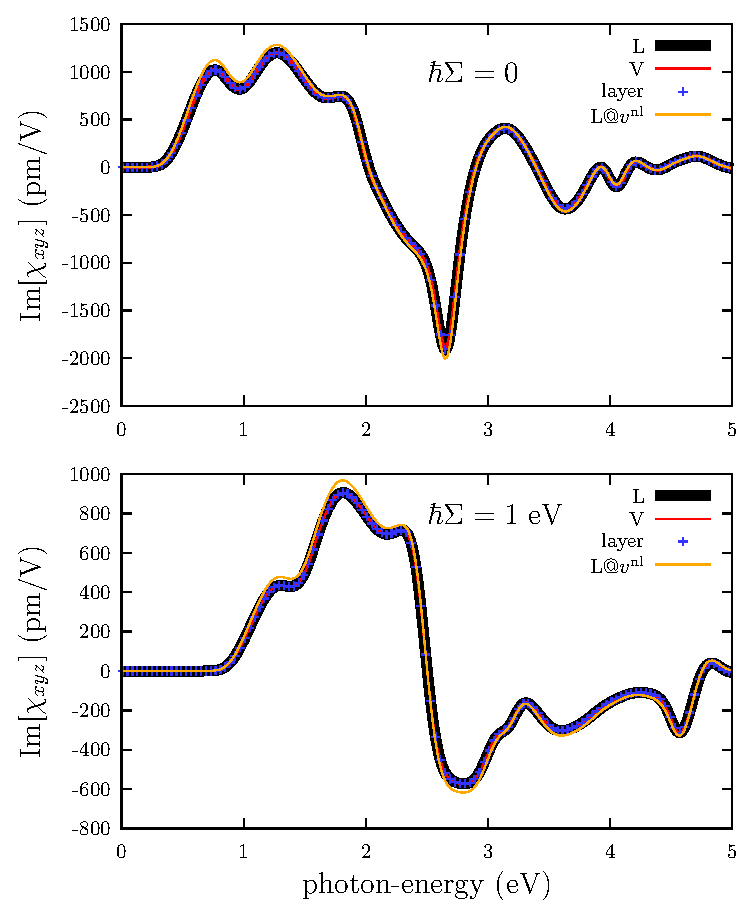
\includegraphics[scale=.7]{content/figures/appendices/shg-bulk}
\caption{Im[$\chi_{xyz}$] for GaAs, 10 Ha and 47 $\mathbf{k}$-points, using the
layered formulation and mimicking a bulk. The correction due to
$\mathbf{v}^\mathrm{nl}$, also agrees with the velocity and the layered approach
(not shown in the figure for clarity).}
\label{gaas}
\end{figure}


\subsubsection{Consistency check-up 2}

In Fig.~\ref{si111as} we show
Im[$\chi_{xx}$] for a surface, where the 
The full-slab result is twice the half-slab
result, with or without $\mathbf{v}^\mathrm{nl}$,  as it must be. Also, the scissors
correction rigidly shifts the spectrum by $\hbar\Sigma$ as it should be.  

\begin{figure}[b]
\centering
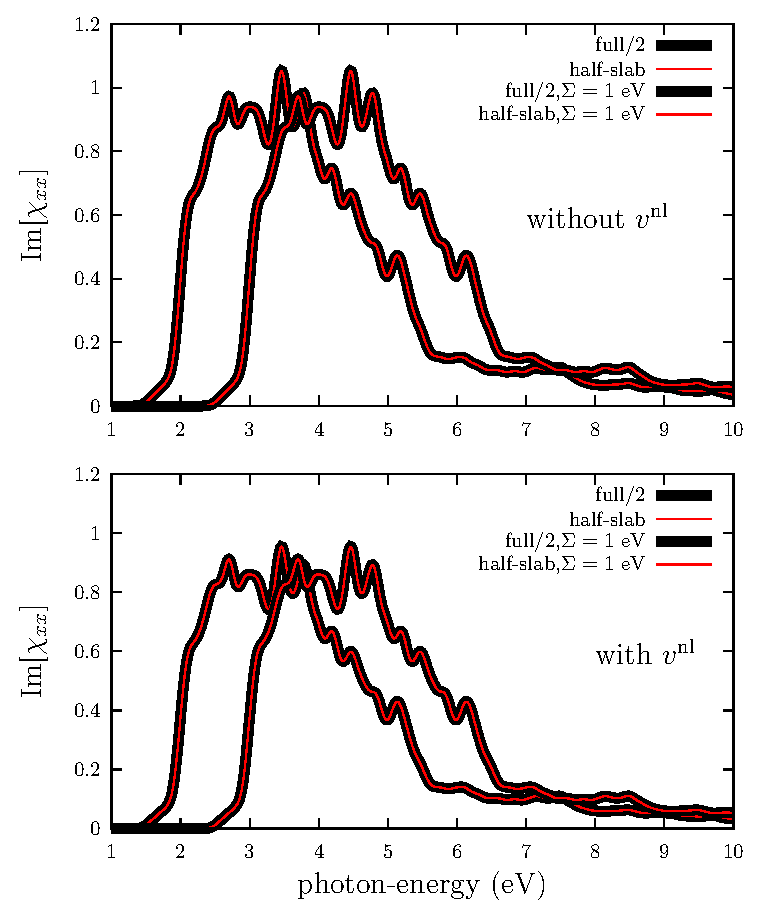
\includegraphics[scale=.7]{content/figures/appendices/surface-chi}
\caption{Im[$\chi_{xx}$] for a Si(111):As surface of 6-layers, 5 Ha and 14
$\mathbf{k}$-points using the layered formulation. The full-slab result is twice
the half-slab result, as it must be. }
\label{si111as}
\end{figure}

\subsubsection{Consistency check-up 3}

Check-of-Checks: 
A (100) $2\times 1$ surface has $\chi_{xxx}$
 different from zero,
whereas the ideally terminated (100) surface has $\chi_{xxx}=0$.
Clean Si(100) has the $2\times 1$ surface as a possible
reconstruction. Then, to calculate such a surface, one can use
a slab such that its front surface is the reconstructed 
Si(100)$2\times 1$ surface and its back surface is H-terminated.
Therefore,
 for the
layer-by-layer scheme one should expect that
\begin{align}\label{cc3}
\chi^{\mathrm{half-slab}}_{xxx}
\equiv
\chi^{\mathrm{full-slab}}_{xxx}
,
\end{align}
since the contribution from the back surface (H-terminated), would
have zero contribution, since this tensor component of $\chi$ is
symmetry forbidden. Fancy at
Fig.~\ref{si-2x1}, and notice that $\chi^\mathrm{nl}<\chi$. i.e. the
susceptibility with the inclusion of the non-local part of the
pseudopotential is smaller than that without it.\\
King-of-Kings: Rejoice at 
Fig.~\ref{si-2x1-n-vs-b}.

\begin{figure}[b]
\centering 
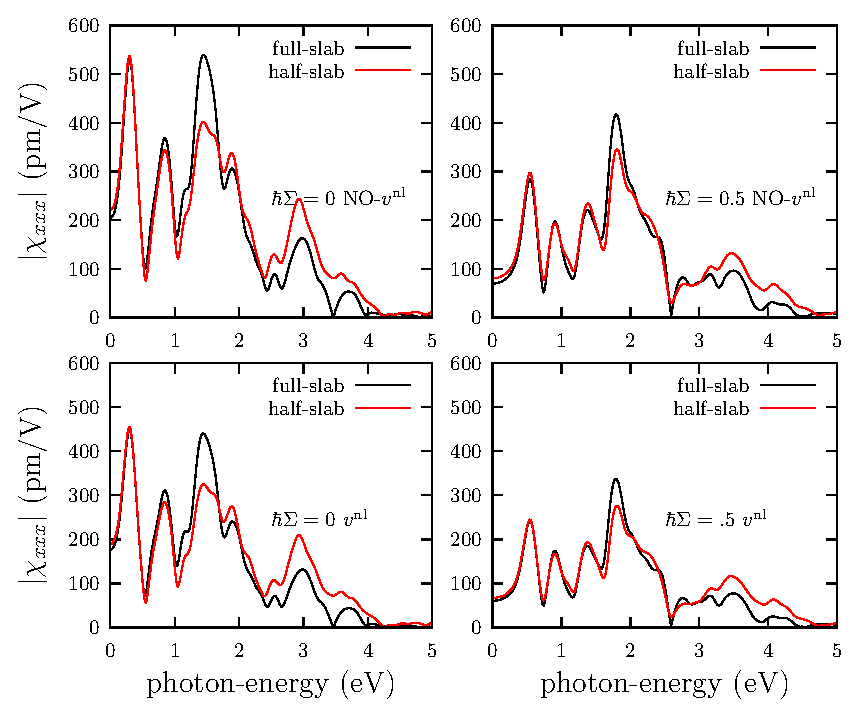
\includegraphics[scale=.7]{content/figures/appendices/shg-si-2x1-16}
\caption{$|\chi_{xxx}|$ for a Si(100)$2\times 1$ surface of 16 Si-layers and one
H layer, 10 Ha, 132 bands,  244 $\mathbf{k}$-points, and 1000 pwvs in DP , using
the layered formulation. We see that $\chi^{\mathrm{half-slab}}_{xxx} \sim
\chi^{\mathrm{full-slab}}_{xxx}$, validating the layer-by-layer approach.}
\label{si-2x1}
\end{figure}

\begin{figure}[b]
\centering
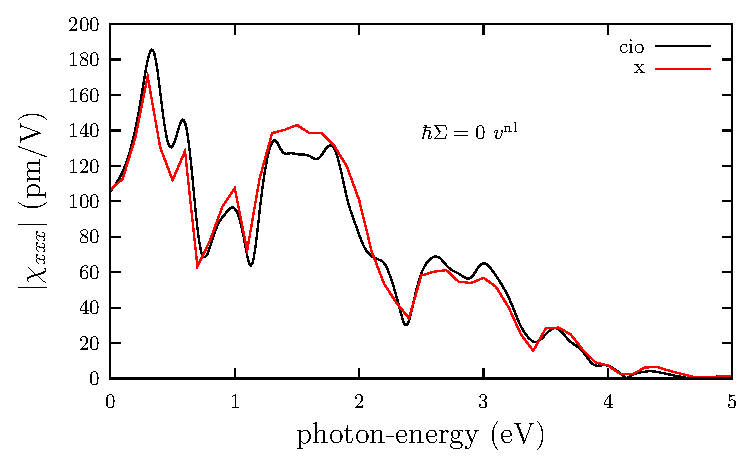
\includegraphics[scale=.7]{content/figures/appendices/shg-si-2x1-n-vs-b}
\caption{$|\chi_{xxx}|$ for a Si(100)$2\times 1$ surface of 12 Si-layers and one
H layer, 5 Ha, 100 bands and 244 $\mathbf{k}$-points for the CIO-TINIBA-coding
and 256 $\mathbf{k}$-point for the X-DP-coding. Both broadened by
0.1 eV. }
\label{si-2x1-n-vs-b}
\end{figure}

\begin{figure}[b]
\centering 
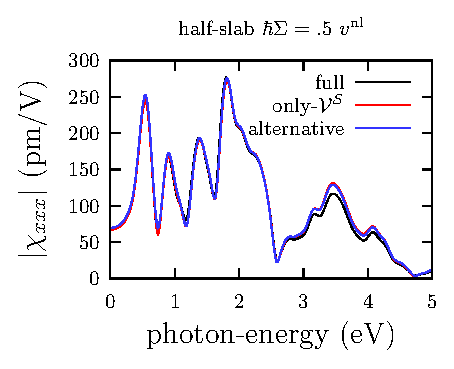
\includegraphics[scale=1.5]{content/figures/appendices/shg-si-2x1-16-compa}
\caption{$|\chi_{xxx}|$ for a Si(100)$2\times 1$ surface of 16 Si-layers and one
H layer, 10 Ha, 132 bands, 244 $\mathbf{k}$-points and and 1000 pwvs in DP,
using the layered formulation. ``Full'' uses full coding of
$\mathcal{V}^\mathcal{S}_{nm}$ and $\mathcal{V}^\mathcal{S}_{nm:\mathbf{k}}$
through Eq.~\eqref{a.3b}; ``only-$\mathcal{V}^\mathcal{S}$'' uses
$\mathcal{V}^\mathcal{S}_{nm}$ through Eq.~\eqref{a.3b} and
$\mathcal{V}^\mathcal{S}_{nm:\mathbf{k}}$ through Eq.~\eqref{ccu55};
``alternative'' uses $\mathcal{V}^\mathcal{S}_{nm}$ through Eq.~\eqref{temp.1}
and $\mathcal{V}^\mathcal{S}_{nm:\mathbf{k}}$ through Eq.~\eqref{ccu55}. Also,
we show the results for 2000 pwvs. Notice that all the curves are almost
identical to each other. }
\label{si-2x1-compa}
\end{figure}

\subsubsection{Consistency check-up 4}\label{ccu4}

To check that the coding of $\mathcal{C}^\ell_{nm}(\mathbf{k})$ is correct, we
can calculate $\mathcal{V}^{\mathrm{a},\ell}_{nm}(\mathbf{k})$ using
Eq.~\eqref{vcali} as follows
\begin{align}\label{ccu.1}
\mathcal{V}^{\mathrm{a},\ell}_{nm}(\mathbf{k})
&=
\frac{1}{2m_e}
\Big(
\mathcal{C}^\ell(z)p^\mathrm{a}
+
p^\mathrm{a}\mathcal{C}^\ell(z)
\Big)_{nm}
\nonumber\\
&=
\frac{1}{2m_e}
\sum_q
\Big(
\mathcal{C}^\ell_{nq}p^\mathrm{a}_{qm}
+
p^\mathrm{a}_{nq}\mathcal{C}^\ell_{qm}
\Big)
,
\end{align}
which must give the same results as those computed through
Eq.~\eqref{eni.2}.
Indeed, we have checked that this is the case. The
\verb=$TINIBA/util/consistency-of-cfmn.sh=
is used to check this.

\subsubsection{Consistency check-up 5}\label{ccu5}

When the \verb=-n= option is chosen, using \verb=all_responses.sh= as
coded above doesn't give consistent results, i.e. $\chi$
 with $\mathbf{v}^\mathrm{nl}$  
is not smaller than $\chi$ 
 without $\mathbf{v}^\mathrm{nl}$. Thus, we follow the bellow approach instead.

We use Eq.~\eqref{nmesn}
\begin{align}\label{nmesnn}
(\mathcal{V}^{\mathrm{LDA},\mathrm{a}}_{nm})_{;k^{\mathrm{b}}}&=
\frac{\hbar}{m_e}\delta_{\mathrm{a}\mathrm{b}}
C^\ell_{nm} 
-i 
\sum_p 
[r^{\mathrm{b}},v^{\mathrm{nl},\mathrm{a}}]_{np}C^\ell_{pm} 
+i 
\sum_{\ell}
\bigg(
r^{\mathrm{b}}_{n\ell}  
\mathcal{V}^{\mathrm{LDA},\mathrm{a}}_{\ell m}
-
\mathcal{V}^{\mathrm{LDA},\mathrm{a}}_{n\ell}   
r^{\mathrm{b}}_{\ell m}
\bigg)  
+i  
r^{\mathrm{b}}_{nm}
\tilde\Delta^{\mathrm{a}}_{mn}
,
\end{align}  
where 
\begin{eqnarray}\label{tdeln}
\tilde\Delta^{\mathrm{a}}_{mn}
=
\mathcal{V}^{\mathrm{LDA},\mathrm{a}}_{nn}  
-
\mathcal{V}^{\mathrm{LDA},\mathrm{a}}_{mm}  
, 
\end{eqnarray}
which is coded instead of Eq.~\eqref{c-a.2nn}. 
 As mentioned before, the term $[r^{\mathrm{b}},v^{\mathrm{nl},\mathrm{a}}]_{nm}$
calculated in Appendix \ref{app:calt}, is small 
compared to the other terms, thus we neglect it throwout this work.\cite{valerie} 
The expression for $C^\ell_{nm}$ is calculated in Appendix \ref{app:calpcalc}.

Likewise, with the help
of Eq.~\eqref{a_gradw2} into
Eq.~\eqref{c-choni.1}, we obain
\begin{align}\label{ccu54}
(v^{\mathcal{S},\mathrm{a}}_{nm})_{;k^\mathrm{b}}&=
i\Sigma f_{mn}(r^\mathrm{a}_{nm})_{;k^\mathrm{b}}
=
i\Sigma f_{mn}\left(\frac{v^{\mathrm{LDA},\mathrm{a}}_{nm}}{i\omega^\mathrm{LDA}_{nm}}\right)_{;k^\mathrm{b}}
\nonumber\\
&=
\Sigma\frac{f_{mn}}{\omega^\mathrm{LDA}_{nm}}\left[
\left(v^{\mathrm{LDA},a}_{nm}\right)_{;k^\mathrm{b}}
-
\frac{v^{\mathrm{LDA},a}_{nm}}{\omega^\mathrm{LDA}_{nm}}\left(\omega^\mathrm{LDA}_{nm}\right)_{;k^\mathrm{b}}
\right]
\nonumber\\
&=
\Sigma\frac{f_{mn}}{\omega^\mathrm{LDA}_{nm}}\left[
\left(v^{\mathrm{LDA},a}_{nm}\right)_{;k^\mathrm{b}}
-
\frac{\Delta^{b}_{nm}}{\omega^\mathrm{LDA}_{nm}}v^{\mathrm{LDA},a}_{nm}
\right]
,
\end{align}
which is generalized as follows 
\begin{align}\label{ccu55}
(\mathcal{V}^{\mathcal{S},\mathrm{a}}_{nm})_{;k^\mathrm{b}}&=
\Sigma\frac{f_{mn}}{\omega^\mathrm{LDA}_{nm}}\left[
\left(\mathcal{V}^{\mathrm{LDA},a}_{nm}\right)_{;k^\mathrm{b}}
-
\frac{\Delta^{b}_{nm}}{\omega^\mathrm{LDA}_{nm}}\mathcal{V}^{\mathrm{LDA},a}_{nm}
\right]
,
\end{align}
although, I haven't found a way to prove this rigorously, it gives 
very similar results to those obtained by Eq.~\eqref{c-a.3bnn}, which 
is coded. 
%which is coded instead of 
The following is also tempting,
\begin{align}\label{temp.1}
v^{\mathcal{S},a}_{nm}
&=\Sigma\frac{f_{mn}}{\omega^\mathrm{LDA}_{nm}}
v^{\mathrm{LDA},a}_{nm}
\nonumber\\
\mathcal{V}^{\mathcal{S},a}_{nm}
&=\Sigma\frac{f_{mn}}{\omega^\mathrm{LDA}_{nm}}
\mathcal{V}^{\mathrm{LDA},a}_{nm}
.
\end{align}
Again, I haven't found a way to prove this rigorously, but it gives 
very similar results to those obtained by Eq.~\eqref{a.3b}, which 
is coded. In Fig.~\ref{si-2x1-compa} we show the comparison between
the two alternatives, from where we see that they are basically equivalent. 


%%%%%%%%%%%%%%%%%%%%%%%%%%%%%%%%%%%%%%%%%%%%%%%%%%%%%%%%%%%%%%%%%%%%%%%%%%%%%%%%
%%%%%%%%%%%%%%%%%%%%%%%%%%%%%%%%%%%%%%%%%%%%%%%%%%%%%%%%%%%%%%%%%%%%%%%%%%%%%%%%

\section{Coding the SSHG yield}

Github repository (\url{https://github.com/roguephysicist/SHGYield})

\begin{figure}
\centering 
\includegraphics[scale=0.9]{content/figures/code-shgyield}
\caption{A simplified example of using Python code to calculate
$\mathcal{R}_{sP}$.}
\label{fig:code-shgyield}
\end{figure}


\stopcontents[chapters]

